% !TEX root =  ../thesis.tex

Before being able to understand how profiles change in time and find anomalous profiles and transactions, we need to understand how a profile is defined and computed.

After preliminary definitions and an explanation of the different types of profiles, we will focus more on their mathematical representation (the histogram) and its properties, with the objective of defining a distance function able to satisfy our requirements.

\section{Definition of User Profile}

In order to define a User Profile, we will first introduce a few preliminary definitions.

\begin{description}
  \item[user] a single client of the bank, be it a private or a company, identified by a unique code in the dataset.
  \item[feature] a dimension of a transaction, which can be of type Integer, Real or Categorical
  \item[window] a period of time on which transactions are grouped and a profile is defined. For each window, only one profile exists, and vice versa. Windows in this thesis will in general be of one month.
  \item[bin selection] the procedure of mapping a value to a bin in a histogram
\end{description}

A profile is computed from a set of transactions that belong to the same time window, and it is composed of a set of histograms, one for each feature. The sum of each histogram is equal to the total number of transactions. Each histogram is composed of 2 or more bins, where the value of each bin is defined as the number of transactions for which the value of the feature related to the histogram is included in the set of bin values.

\subsection{Histograms and their properties}

Now we shift the focus from the overall user profile to the properties of a single histogram. A single histogram represent a pattern in the user transactions over that feature. For instance, let us take the feature `amount' in consideration. The amount is simply the monetary value of a transaction, expressed in euros. A histogram mostly flat, such as in figure \ref{fig:flat_histogram}, means that the user makes transactions of all amounts indiscriminately. If the histogram is mostly skewed to the left, the user will prefer smaller transactions; if to the right, bigger transactions.

\begin{figure}[h]
\centering
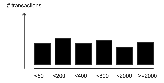
\includegraphics[width=250]{images/flat_histogram.pdf}
\caption{Histogram representing the distribution of transactions over the `amount' feature}
\label{fig:flat_histogram}
\end{figure}

To understand this, only the shape of the histogram is relevant, and can therefore be normalized to have sum one and interpreted as a dicrete probability distribution.

We refer to a histogram with the notation $H$, and to the value of bin $i$ with $H(i)$.

We follow the classification of histograms as proposed in \cite{histogram}, which divides histograms in three families based on their type of measurement:

\begin{description}
\item[ordinal] the values are ordered, such as numbers or more in general anything that can be ordered.
\item[nominal] the values are a finite set of possible categories, without any ordering implied.
\item[modulo] the values are ordered in a `ring' where the rightmost values are close to the leftmost ones, as in the arithmentic modulo operation.
\end{description}

\section{Distance between histograms}

In order to compute how profiles change over time, we need to introduce the concept of a distance between histograms. This topic is central to this thesis, and will be explored in depth, as it provides the basis for the whole temporal profile analysis system.

We refer to the distance between histgrams $H(A)$ and $H(B)$ as $d(H(A), H(B))$
The distance function will need to be specified over histograms of the same family, and possibly be specialized for each one. It will need to satisfy the following properties:
\begin{description}
  \item[symmetric] $d(H(A), H(B)) = d(H(B), H(A))$
  \item[positional] for ordinal and modulo histograms, the distance between bins should be taken into account
\end{description}

While the first property is self explanatory, the second one requires further explanation. Take as an example the following three histograms:\\
$H(A) = [1, 0, 0, 0, 0]$\\
$H(B) = [0, 1, 0, 0, 0]$\\
$H(C) = [0, 0, 0, 0, 1]$

The desired behavior will depend on the type of these histograms:
\begin{description}
  \item[nominal] all distances should be equal
  \item[ordinal] $d(H(A), H(B)) < d(H(A), H(C))$ since the bins containing a 1 are further apart in the second case
  \item[modulo] $d(H(A), H(B)) = d(H(A), H(C))$ since the bins containing a 1 are next to each other, if we see the histogram as a ring
\end{description}

We say that the distance is \textit{shuffling invariant} for nominal histograms and \textit{shuffling dependent} for ordinal and modulo histograms.

This property is clearly desirable for our scenario, where a shift in spending habits from transactions around 500 euros to transactions around 800 euros is less relevant than a shift to transactions around 5000 euros. Also, we want to be able to tune this dependence to shuffling so that histograms built on different features can consider the distance between bins independently.

Unfortunately, the typical ways used to measure histogram distance do not satisfy our required properties. In the following sections we will analyze a few possible distances and finally define a new distance function that suits our purposes.

\subsection{Vector representation based distances}

A typical way to define distances is to see histograms as vectors and apply typical vector distances. A few common distances are:
\begin{description}
  \item[city block] sum over each dimension $i$ of $|H(A,i) - H(B,i)|$
  \item[euclidean] squared sum over each dimension $i$ of $(H(A,i) - H(B,i))^2$
\end{description}

As with all vector based distances, these distances are shuffling invariant ad not enough for what we need.

%\subsection{DPDF representation based distances}

%If se see each histogram as a DPDF (discrete probability density function) we can use probabilistic measures of distances. Good measures would be:
%\begin{description}
  %\item[Bhattacharyya distance] TODO
  %\item[Matusita distance] TODO
  %\item[K–L distance] TODO
%\end{description}

\subsection{Miminum distance of pair assignments}

The MDPA (minimum distance of pair assignments) is a distance function defined in \cite{histogram} that almost satisfies our requirements. To define the MDPA consider two sets of n elements, A and B, which define histograms $H(A)$ and $H(B)$. The MDPA is intuitively equal to the minimum total cost of the `moves' that we need to make in order to transform the first histograms in the second one. A move is defined as subtracting $x$ from bin $i$ and adding it to bin $j$. The cost of a move is $x * d(i, j)$ where $d(i, j)$ is the linear distance between the two bins.

This distance can be used for ordinal and modulo histograms as it takes into account the position of bins. Moreover, efficient algorithms exist for computing the MDPA distance. However, the problem is that in these algoritms the distance $d(i, j)$ between bins is considered to be a linear distance. We think that this is not acceptable in our scenario, since the meaning of such distance depends on the feature measured by the profile associated with the histogram and other distances could be necessary. In particular, exponentially decreasing distances could make more sense in real world situations, where for instance $d(i, j), i=0, j=4$ should be more than double than $d(i, j), i=0, j=2$.

Defining a custom distance $d(i, j)$ that is non linear is possible in MDPA, but leads to a generic linear optimization problem with exponential complexity. Because of this, we decided to discard the MDPA distance and opt for a completely different approach, as explained in the following section.

\section{Filter \& measure approach}

Our approach is based on a completely different technique: instead of finding a distance algorithm that takes bin position into account, we apply a `blurring' filter to the histograms and then apply a standard vector distance, such as the euclidean distance.

The blurring filter we decided to use is the gaussian smoothing filter, where each bin in the smoothed histogram is the weighed average of its surrounding bins, using the gaussian function to compute the weights.

The gaussian function with mean $\mu = 0$ is defined as:
\begin{displaymath}
  \frac{1}{\sigma\sqrt{2\pi}}e^{-\frac{x^2}{2\sigma^2}}
\end{displaymath}

For instance, the weight assigned in the weighed average to a bin next to the one being computed is given by the gaussian function where $x = 1$, being $x$ the distance between the bins. Usually we consider as insignificant bins with distance $x > 3\sigma$.

This method can account for different types of histograms and can be tuned by adjusting the parameter $\sigma$ of the gaussian function in order to specify how much the histograms should be smoothed before computing their euclidean distance.

In particular, we have as always three types of histograms to account for:

\begin{description}
  \item[nominal] no smoothing should be applied, the euclidean distance can be computed directly
  \item[ordinal] smoothing should be applied, if the weighed average would includes bins outside of the histogram range (for instance, when computing the average for the first or last bin) it should be limited to those available.
  \item[modulo] smoothing should be applied, but in this case when bins are outside of the histogram range they will be taken from the other end of the histogram, following the rules of the arithmentic modulo operator.
\end{description}

\subsection{Example of the filter \& measure approach}

Let us take two histograms, $H(A)$ and $H(B)$ defined as:
\begin{align}
  H(A) = [1,5,7,2,3,9,2]\\
  H(B) = [0,3,6,2,1,2,1]
\end{align}

The first step to compute the distance is to process these histograms with a smoothing filter, as previously explained. To understand the effects of such filtering, look at figure \ref{fig:sigma_difference}. The original histogram, printed in black, is $H(A)$. In green we can see the smoothed version of the histogram, on the left with $\sigma = 0.5$ and on the right with $\sigma = 1$. As you can see, raising the value of the $\sigma$ parameter increases the smoothing effect.

\begin{figure}[h]
\centering
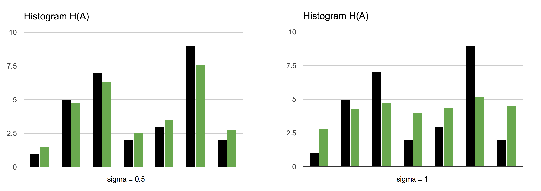
\includegraphics[width=450]{images/sigma_difference.pdf}
\caption{In green the smoothed version of the histogram in black, for two different values of the $\sigma$ parameter}
\label{fig:sigma_difference}
\end{figure}

In figure \ref{fig:smoothed_a_b} we can see the two histograms along with their smoothed version at $\sigma = 0.5$. The final distance will be the euclidean distance between the smoothed version. These are the distances at different smoothing levels:
\begin{align}
  \sigma = 0.5, \text{distance} = 6.91\nonumber\\
  \sigma = 1, \text{distance} = 6.09\nonumber\\
  \sigma = 2, \text{distance} = 5.53\nonumber
\end{align}
Without smoothing the distance would have been $7.74$, higher than any of the other distances. This is because, thanks to smoothing, we can take into account the fact the similarity of values in close bins. For instance, take $H(A,1) = 1$ which became $H(A,1) = 0.4$ after smoothing, thanks to the presence of the bin next to it which had a value of $3$.

\begin{figure}[h]
\centering
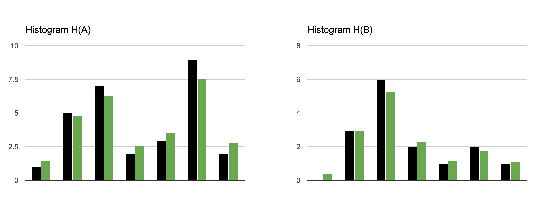
\includegraphics[width=450]{images/smoothed_a_b.pdf}
\caption{Original and smoothed versions of the two histograms $H(A)$ and $H(B)$ at $\sigma = 0.5$}
\label{fig:smoothed_a_b}
\end{figure}

